\documentclass{article}

\usepackage[final]{style}
\usepackage[utf8]{inputenc} % allow utf-8 input
\usepackage[T1]{fontenc}    % use 8-bit T1 fonts
\usepackage{hyperref}       % hyperlinks
\usepackage{url}            % simple URL typesetting
\usepackage{booktabs}       % professional-quality tables
\usepackage{amsfonts}       % blackboard math symbols
\usepackage{nicefrac}       % compact symbols for 1/2, etc.
\usepackage{microtype}      % microtypography
\usepackage{verbatim}
\usepackage{graphicx}       % for figures

\title{Lecture \#6: Advanced Policy Gradients}

\author{
  Chong Yihui, Shen Ting, Dongyang\\
  Department of Computer Science\\
  National University of Singapore\\
  Singapore, S117417 \\
  \texttt{\{ychong, STUDENT2, etc.\}@u.nus.edu} \\
}

\begin{document}

\maketitle


\section{Policy gradient as policy iteration}
First, we try to show that we can use the advantage of the previous policy to get a better policy and the result method looks like policy gradient.

To do so, we try to maximise the difference in the returns: $J(\theta') - J(\theta)$

We claim the following equivalence:

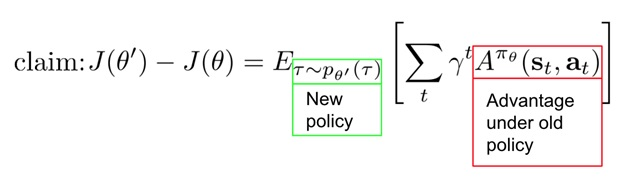
\includegraphics[scale=0.5]{claim1.jpg}

Recall that $J(\theta) = E_{{s_0}\sim p(s_1)}}[V^{\pi_\theta}(s_0)}]$

The following derivation tricks are used:

1. Initial state distribution is the same for all policy.

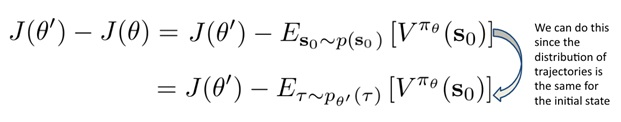
\includegraphics[scale=0.5]{claim1_1.jpg}

2. Expanding out $V^{\pi_\theta}(s_0)}$ to a telescoping sum 

$V^{\pi_\theta}(s_0)} = \sum_{t=0}^{\infty}\gamma^tV^{\pi_\theta}(s_t) - \sum_{t=1}^{\infty}\gamma^tV^{\pi_\theta}(s_t)$

$=V^{\pi_\theta}(s_0)+\gamma^1V^{\pi_\theta}(s_1)+\gamma^2V^{\pi_\theta}(s_2)...-[\gamma^1V^{\pi_\theta}(s_1)+\gamma^2V^{\pi_\theta}(s_2)+...]$

3. Correction: t=0 instead of t=1 for $J(\theta)$

$J(\theta') = E_{{\tau}\sim p_{\theta'}(\tau)}}[\sum_{t=0}^{\infty}\gamma^{t}r(s_t,a_t)]$ 

instead of 

$E_{{\tau}\sim p_{\theta'}(\tau)}[\sum_{t=1}^{\infty}\gamma^{t}r(s_t,a_t)]]$

After using the above trick, we would have proofed our claim. Next, we instead of taking expectation over our new policy(which we do not have yet and is what we are trying to find), we would like to take the expectation over the old policy.

\section{Ignoring distribution mismatch}

$E_{{\tau}\sim p_{\theta'}(\tau)}[\sum_{t}\gamma^{t}A^{\pi_\theta}(s_t,a_t)] = \sum_{t}E{s_t\sim p_{\theta'}(s_t)}[E{a_t\sim \pi_{\theta'}(a_t|s_t)}[\gamma^t A^{\pi_\theta}(s_t,a_t)]]$

Using importance sampling we are able to switch the inside expectation to get the following equation:
$= \sum_{t}E{s_t\sim p_{\theta'}(s_t)}[E{a_t\sim \pi_{\theta}(a_t|s_t)}[\frac{\pi_{\theta'}(a_t,s_t)}{\pi_{\theta}(a_t,s_t)}\gamma^t A^{\pi_\theta}(s_t,a_t)]]$

However, we are not able to do this for the outer expectation as
$\frac{\pi_{\theta'}(a_t,s_t)}{\pi_{\theta}(a_t,s_t)} < 1$ and the probability of state is a series of multiplication. Therefore, the importance sampling weight decays to 0 as the time horizon gets longer.

Main Takeaway: we can use our existing policy to approx our cost if they are similar (ignore the distribution mismatch)
Next, under what conditions are they similar?

\section{Bounding the distribution change}
Important notation: $|p_{\theta'}(s_t) - p_\theta(s_t)| = \sum_x(|p(x) - q(x)|)$

Also note that $|p_{\theta'}(s_t) - p_\theta(s_t)| <= 2$.

A possible worst case: Consider 2 different points $x_1, x_2$ such that
$p(x_1) = 1$ and $q(x_1) = 0$

$p(x_2) = 1$ and $q(x_2) = 0$

$|p_{\theta'}(s_t) - p_\theta(s_t)| = |1 - 0| + |0 - 1| = 2$

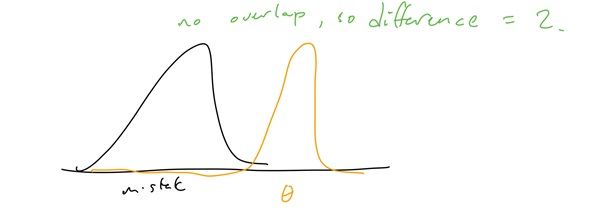
\includegraphics[scale=0.5]{bounding_dist2.jpg}

When can we change $p_{\theta'}$ to $p_\theta$?

[Case 1: Assume policy is deterministic]
Claim: $p_\theta(s_t)$ is close to $p_\theta'(s_t)$ when $\pi_\theta$ is close to $\pi_\theta'$

Definition of close for deterministic distribution:

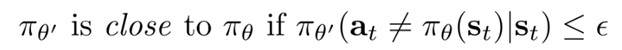
\includegraphics[scale=0.5]{bounding_dist1.jpg}

If the above bound holds,

$|p_{\theta'}(s_t) - p_\theta(s_t)| \leq 2\epsilon t$
\newline\newline

[Case 2: Assume policy is stochastic]

Definition of close for general case:

$\pi_{\theta'}$ is close to $\pi_\theta$ if  $|\pi_{\theta'}(at|s_t) - \pi_\theta(at|s_t)| \leq \epsilon$ for all $s_t$

If the above bound holds and using the useful lemma,

$|p_{\theta'}(s_t) - p_\theta(s_t)| \leq 2\epsilon t$

\section{Bounding with KL-divergence}

Instead of using $\epsilon$ in the above bound, we can also bound the policy using KL-divergence 

$|\pi_{\theta'}(at|s_t) - \pi_\theta(at|s_t)| \leq \sqrt{\frac{1}{2}D_{KL}(\pi_{\theta'(a_t|s_t)}||\pi_\theta(a_t|s_t))}$\\

With this, we get the following objective function

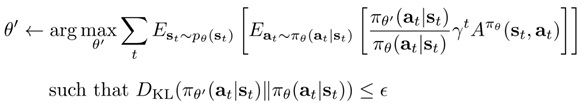
\includegraphics[scale=0.5]{kl-div.jpg}

To optimize the above objective, 

[Method 1] Enforce the constraint on the KL divergence use Lagrangian method. 

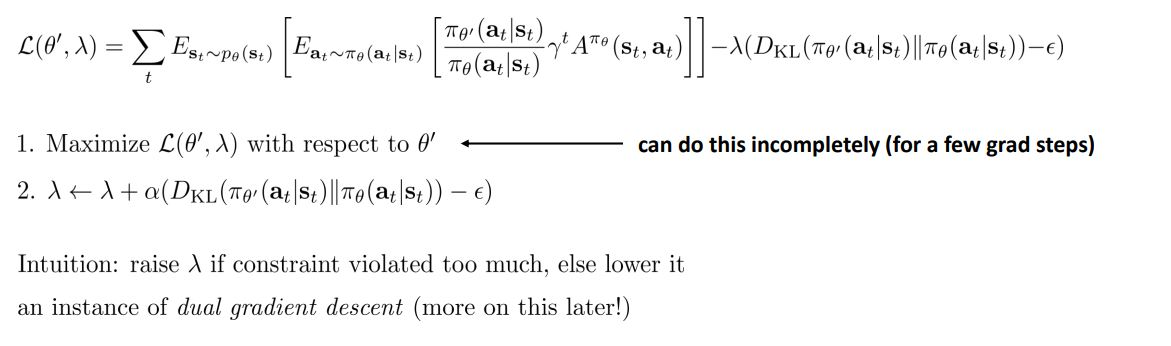
\includegraphics[scale=0.5]{lagrange_f.jpg}

This is an example of dual gradient descent (on both $\theta$ and $\lambda$)

[Method 2] Use natural policy gradient (for further reading). 

[Method 3] Use natural policy gradient with learning rate (Trust region policy optimization)

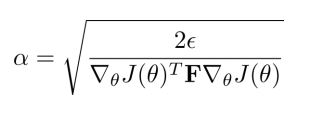
\includegraphics[scale=0.5]{trust_lr.jpg}

\section{Further Readings}
Going towards the trust region policy gradient algorithm:

\url{https://medium.com/@jonathan_hui/rl-natural-policy-gradient-actor-critic-using-kronecker-factored-trust-region-acktr-58f3798a4a93}

Trust Region Policy Optimization (TRPO) using Adam

\url{https://medium.com/@jonathan_hui/rl-trust-region-policy-optimization-trpo-part-2-f51e3b2e373a}\\

Natural Gradient and Fisher Information: 

\url{https://wiseodd.github.io/techblog/2018/03/11/fisher-information/}

\url{https://wiseodd.github.io/techblog/2018/03/14/natural-gradient/}\\


Natural Gradient Intuition

\url{ http://kvfrans.com/a-intuitive-explanation-of-natural-gradient-descent/}\\

Intuitive explanation of Policy Gradients

\url{http://karpathy.github.io/2016/05/31/rl/
}
% References
\small
\bibliographystyle{plain}
\bibliography{bibliography}
\end{document}
